\chapter{Estimação dos juros em projetos de software livre}

Neste capículo descreveremos uma instância do modelo de estimação dos juros da dívida técnica descrito no Capítulo \ref{estimacao:juros}. Essa instância será criando observando as particularidades relacionadas aos projeto de software livre.  

\section{Introdução}

Conforme descrito no Capítulo \ref{estimacao:juros}, são necessários quatro definições para a criação de uma instância do modelo abstrato de estimação dos juros: Métricas de entrada, métricas de saída, método de agrupamento e método de particionamento. A seguir definiremos cada um desses itens observando as principais características dos projetos de software livre. Um dos motivos para termos escolhido esse tipo de projeto foi a facilidade que teremos para obter os dados necessários para o estudo de caso que realizaremos nos Capítulos \ref{cap_estudo_caso} e \ref{cap_estudo_caso_execucao}. Além disso, acreditamos que indicar uma forma de estimar os juros seja uma contribuição relevante para a comunidade de software livre.

\section{Entradas}
\label{cap_metodo:modelos_de_entrada}

Consideraremos a contribuição dos colaboradores dos projetos como a entrada do nosso modelo de avaliação da produtividade. Essa característica foi a escolhida para representar a entrada do modelo de análise de produtividade já que a colaboração é o que efetivamente faz com que  o projeto de software livre possa evoluir. O esperado é que quanto mais colaboração um projeto tiver, mais ele estará apto a atingir seus objetivos. 

Existe uma particularidade nos projetos de software livre em relação ao que é gasto  para que o software seja construído. Nesse tipo de projeto, normalmente, não há uma relação profissional entre os colaboradores e a empresa ou organização interessada no desenvolvimento do software. Em vez disso, essa colaboração é feita voluntariamente, seja porque o colaborador tem interesse nas funcionalidades fornecidas pelo software sendo construído seja porque ele deseja aprender mais a respeito das tecnologias utilizadas, insto é, por qualquer outro motivo. 

Não há, no contexto do software livre, normalmente, uma relação que envolva um pagador e um recebedor. Logo, não podemos identificar os gastos que uma organização teve para manter a equipe de funcionários que realizou o projeto já que não existe uma organização e também não existem funcionários. Ainda assim, podemos atribuir esse dois papéis (organização e funcionário), respectivamente,  para a comunidade de colaboradores e os colaborares em si. 

Podemos considerar que a comunidade de colaboradores está investindo recursos ao alocar colaboradores para contribuir com um projeto. Mesmo sabendo que essa alocação não parte de uma unidade específica, mas ao invés disso, é realizada por meio da vontade individual de cada colaborador. Com isso, podemos estimar a produtividade de um projeto ao medir o quanto de colaboração esse projeto obteve e o quanto de retorno essa colaboração gerou. Projetos que obtiveram muita colaboração e pouco retorno serão considerados improdutivos , enquanto que projetos com pouca colaboração e muito retorno serão considerados produtivos. A forma de medir qual o retorno que um projeto forneceu à comunidade será descrita na seção \ref{secao_modelo_concreto_saidas}.

Utilizaremos três modelos diferentes para calcular o nível de colaboração de um projeto:

\begin{itemize}

\item \textbf{Homens/Dia}. Uma das formas comuns de medir esforço é utilizando a quantidade de homens por hora empregados em um projeto. Como no contexto do software livre dificilmente teremos acesso à quantidade de horas que um colaborador contribuiu, utilizamos a quantidade de dias. 

\item \textbf{Quantidade de colaboradores}. Testaremos também um modelo mais simples que não leva em consideração nenhum atributo adicional a respeito do colaborador. Iremos apenas contar a quantidade de pessoas que contribuíram para o projeto e usar isso como a entrada do modelo de produtividade.
\item \textbf{Assiduidade e qualidade da colaboração}. Nesse modelo consideraremos como a entrada do processo de desenvolvimento de software um índice de colaboração que será calculado por meio da assiduidade em que um determinado colaborador contribui para um projeto e o seu nível de prestígio dentro da comunidade de software. 
\end{itemize}

Utilizamos mais de um modelo, pois, não sabemos qual deles se mostrará mais adequado de acordo com os dados que utilizaremos no estudo de caso no Capítulo \ref{cap_estudo_caso}.

Os três primeiros modelos são simples e não necessitam de maiores esclarecimentos. Já o último modelo é complexo e por isso o descreveremos em detalhes a seguir. 


\subsection{O modelo de assiduidade e qualidade da colaboração}

Nesse modelo a colaboração será medida por meio de dois aspectos:  qualidade e assiduidade. Essa divisão foi realizada com o objetivo de capturar mais detalhes a respeito do custo da colaboração na evolução dos projetos.  É esperado, por exemplo, que utilizando menos tempo, programadores mais experientes darão contribuições mais significativas para projetos complexos do que programadores iniciantes. Dessa forma, o tempo gasto por programadores experientes será mais caro do que o de programadores iniciantes. Esse conceito de custo deve ser observado levando-se em consideração nossa abordagem de pensar no tempo gasto pelos colaboradores como um investimento da comunidade no projeto.  Descreveremos qual  característica cada um desses aspectos irá representar e como eles serão calculados. Por fim, descreveremos a variável índice de colaboração (IC), ela irá agregar esses dois aspectos em uma única métrica.

\subsubsection{Qualidade da colaboração}
\label{cap_modelo_colaboracao_concreto}

Para estimar a qualidade da colaboração que um projeto recebeu iremos estimar o  nível de proficiência do colaborador na linguagem utilizada no projeto. Acreditamos que colaboradores com maior conhecimento nas tecnologias que o projeto utiliza normalmente darão uma contribuição de maior qualidade do que colaboradores com menos conhecimento. O nível de conhecimento de cada colaborador será calculado por meio de uma técnica para classificar colaboradores de acordo com o seu nível de expertise. 

Na literatura, pudemos encontrar algumas abordagens para estimar o nível de expertise de um indivíduo a respeito de um assunto:  

\begin{itemize}
\item Hupa et al.\cite{hupa2010interdisciplinary} sugerem uma abordagem baseada em três dimensões, para avaliar a  habilidades de um colaborador. Essas dimensões são o conhecimento, a confiança e a rede de relacionamento. Os autores então propõem um modelo que utiliza dados a respeito dessas três dimensões. Esse modelo é utilizado para calcular uma estimativa para o desempenho de um time formado pelos colaboradores avaliados.
\item Outra abordagem, dessa vez focada no contexto acadêmico, é o trabalho de Kalaiselvi et al. \cite{kalaiselvi2013ontological}. Nele os autores criaram uma ontologia para identificar a principal área de conhecimento dos membros de uma universidade e estimar o nível de conhecimento desses membros a respeito dessa área.
\item  Outras contribuições relevantes para esse problema são os trabalhos de Mockus et al.\cite{mockus2002expertise} e Shira et al.\cite{shira2011expert}. Nesses dois trabalhos, os autores criam um modelo  e uma ferramenta para encontrar especialistas em repositórios de software. Além de permitir a procura por assunto, essas ferramentas também possibilitam que os usuários possam encontrar colaboradores que sejam especialistas até mesmo em um bloco específico do código de um projeto de software.
\item No contexto das plataformas de desenvolvimento que também possuem funcionalidades de interação social, como é o caso do GitHub e StackOverflow, existem os trabalhos de Huang et al. \cite{huang2017expert}, Munger et al.\cite{munger2014automatically}, Pedro et al.\cite{san2013multiple} e Robber et al.\cite{robbes2013using}. Nesses trabalhos são sugeridas  abordagens que consideram as especificidades  de cada uma dessas plataformas.
\end{itemize}    

Nesta pesquisa utilizaremos,  para estimar o nível de expertise dos colaboradores de um projeto,  a abordagem \textit{GEMiner} que foi sugerida por Mo et al.\cite{mo2015geminer}.  Essa abordagem foi escolhida, dentre as outras disponíveis, pelas seguintes razões:

\begin{itemize}
\item \textbf{É uma abordagem focada na classificação de programadores.} Algumas das outras abordagens encontradas na literatura são gerais e podem ser utilizadas para encontrar especialistas em diferentes domínios de atuação. Entretanto, elas não foram criadas e avaliadas levando em consideração as particularidades da área de desenvolvimento de software. Com isso, pode ser que determinadas características dessa área possam fazer com que essas abordagens produzam resultados incorretos.
\item \textbf{Apresenta uma análise comparativa com trabalhos anteriores.} Na pesquisa desenvolvida por  Mo et al.\cite{mo2015geminer} foi realizada uma série de experimentos para avaliar a eficácia do modelo proposto. Em uma dessas avaliações, foi realizada uma comparação entre o resultado gerado pela aplicação do modelo e uma lista oficial com os programadores mais influentes da linguagem Javascript. A comparação mostrou que houve um alto número de intersecções entre a lista oficial e o resultado gerado pelo modelo. Com isso, os autores puderam concluir que a abordagem sugerida por eles apresenta um nível satisfatório de precisão. 
\item \textbf{A estratégia foi criada e validada considerando as particularidades da plataforma GitHub.} Isso nos garantiu que a aplicação do GEMiner seria possível já que nosso estudo de caso também iria utilizar dados provenientes do GitHub. Esse procedimento foi importante na escolha dessa proposta pois algumas das outras exigiam dados que não estavam disponíveis no GitHub.
\item \textbf{Abordagem simples}. Por ser baseada em um algoritmo muito conhecido, o  PageRank \cite{page1999pagerank},  pudemos compreender e aplicar essa abordagem de forma rápida. Além disso, os modelos matemáticos utilizados pelos autores são intuitivos e bem documentados.
\item \textbf{Uma descrição detalhada a respeito dos modelos matemáticos utilizados.} Em algumas das outras abordagens possíveis para a estimação da expertise, o texto da pesquisa não era claro a respeito dos passos necessários para aplicar o modelo. Em algumas abordagens alguns cálculos não foram descritos com um nível de detalhamento suficiente ou até mesmo alguns passos para a aplicação não foram devidamente descritos. Entretanto, isso não ocorreu com o GEMiner. Os autores descreveram com detalhes cada um dos cálculos necessários. Inclusive fornecendo as fórmulas matemáticas e exemplos de como aplicá-las. Além disso, houve um nível de detalhamento satisfatório durante a apresentação dos experimentos realizados pelos autores. Esse fato nos permitiu adaptar e implementar a estratégia de uma forma muito próxima da original, o que se torna importante pois, caso tivéssemos utilizado uma abordagem muito abstrata, não poderíamos nos respaldar nas validações realizadas pelos autores já que nossa implementação poderia ter sido significativamente diferente da implementação que foi realizada e validada pelos autores.
\item \textbf{Resolve problemas encontrados em abordagens anteriores.} Os autores tiveram o cuidado de analisar os trabalhos anteriores e identificar seus problemas. Uma das preocupações foi a de não considerar um especialista apenas alguém que possua prestígio na rede de colaboradores. Essa abordagem pode acontecer porque o indivíduo possui algum atributo que o faça ser bem visto pelos outros colaboradores. Entretanto, esse atributo não tem necessariamente alguma relação com suas habilidades técnicas. Esse é o caso do perfil do ex-presidente americano Barak Obama na plataforma GitHub. Esse perfil é seguido e bem avaliado por uma grande quantidade de pessoas. Entretanto, o número de contribuições feito por ele é muito pequeno. O GEMiner consegue evitar que perfis como esse sejam incorretamente classificados como especialistas.
\end{itemize}


Conforme dito anteriormente, o GEMiner é baseado no algoritmo PageRank, popularmente conhecido como o algoritmo do Google. O objetivo desse algoritmo é criar uma classificação baseada em uma rede de relacionamentos. No contexto das pesquisas de páginas web, esse relacionamento é formado por links. Uma página \textit{A} está relacionada com uma página \textit{B}, se existe em \textit{A} um link que aponte para \textit{B}. Assim, quanto mais links apontarem para uma determinada página, maior a  chance de que essa página seja relevante e deva ser incluída nos resultados da pesquisa.  

Uma das funcionalidades de interação social presentes no GitHub é  a possibilidade de um colaborador poder seguir outros colaboradores como também ser seguido.  Podemos verificar por meio da Figura \ref{fig:cap_modelo_seguir_seguido} que as relações entre os colaboradores podem ser modeladas como um grafo.

 A relevância de um determinado colaborador na comunidade é medida pela quantidade de pessoas que o seguem. Se um colaborador tem muitos seguidores, isso é um indício de que ele seja um especialista. Entretanto, o PageRank não realiza apenas uma contagem das relações individuais entre os elementos do grafo. Em vez disso, todo o contexto do grafo é considerado. Por exemplo, na Figura \ref{fig:cap_modelo_seguir_seguido} tanto o colaborador $D$ quanto o colaborador $F$ possuem apenas um seguidor. Entretanto, o colaborador $F$ é seguido pelo colaborador $C$ e esse colaborador é seguido por outros quatro colaboradores. Logo, apesar do número de seguidores de $D$ e $F$ ser igual,  o colaborador $F$ será considerado mais relevante do que o colaborador $D$ pois ele é seguido pelo colaborador  $C$ que é o colaborador mais relevante desse conjunto. 

Outra característica importante do PageRank é a de que ele leva em consideração a quantidade de relações de saída de cada elemento. Por exemplo, o colaborador $C$ da Figura \ref{fig:cap_modelo_seguir_seguido} segue apenas o colaborador $F$. Enquanto isso, o colaborador $E$ segue os colaboradores $C$ e $D$. No momento de calcular a relevância dos colaboradores $C$ e $D$, adicionando a eles a relevância de $E$,  o algoritmo dividirá por dois a relevância que o colaborador $E$ possui. Por fim, para evitar problemas durante o cálculo do grafo ao encontrar ciclos como o que vemos entre $D$ e $E$,  foi utilizada uma adaptação sugerida por Richardson et al.\cite{richardson2002intelligent}. Nela, em vez de escolher um nó inicial, realizar os cálculos necessários e depois navegar para os vizinhos até que haja uma convergência, o algoritmo aleatoriamente pode, a cada passo, ir para um vizinho ou escolher qualquer outro nó do grafo. Além de evitar ciclos infinitos como aconteceriam entre os nós $D$ e $E$, essa versão do algoritmo também pode ser utilizada em grafos desconexos. 

  \begin{figure}[H]
  \centering
  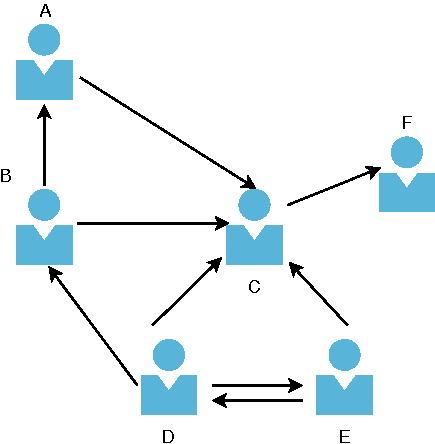
\includegraphics{capitulo_modelo/seguir_seguido.pdf} 
  \caption{As relações de seguir e poder ser seguido no GitHub. Adaptado de \cite{mo2015geminer}.}
  \label{fig:cap_modelo_seguir_seguido} 
\end{figure}

A equação \ref{eq:cap_modelo_equacao1_geminer} é a base do algoritmo PageRank. Como pode ser visto, trata-se de uma equação recursiva. Isso acontece pois para se calcular a relevância de um colaborador é necessário calcular a relevância de todos os colaboradores que o seguem. 

A primeira parte da equação inicializa o \textit{pagerank} de cada elemento ao dividir o número 1 - $d$ pela quantidade de colaboradores em todo o grafo sendo analisado. Sendo que $d$ é o chamado \textit{dumping factor} e indica a probabilidade de que no próximo passo o algoritmo calcule a relevância de um nó adjacente ao atual ou de um nó qualquer aleatório do grafo.  O valor sugerido para  $d$  pelos autores é de 0.85. Os vértices do grafo analisado são representados pelas letras $u$ e $v$. Sendo assim, a equação representa o cálculo da relevância do vértice $v$ e, para isso, realiza uma soma da relevância de todos os outros vértices $u$ de tal forma que $u$ seja $v$. O elemento  $L(u)$ indica quantos outros colaboradores o colaborador $u$ também segue. 

\begin{equation}
\label{eq:cap_modelo_equacao1_geminer}
PR(v) =  \frac{1-d}{\mid V \mid} + d *  \sum_{(u,v) \in E}  \frac{PR(u)}{L(u)}
\end{equation}

Além de considerar o relacionamento ``seguir'' e ``ser seguido'', os autores consideram outros aspectos para avaliar a expertise de um colaborador. Eles nomeiam essa abordagem de \textit{Multi-Source PageRank} já que a classificação é realizada por meio de múltiplos atributos.   O outro aspecto utilizado para avaliar a expertise de um colaborador é o nível de popularidade dos projetos que ele contribuiu. Isso é feito de duas formas, a primeira é analisando quais colaboradores estão observando(\textit{watching}) o projeto. Quanto mais colaboradores relevantes observam um determinado projeto, maior é a relevância dele. A segunda forma de avaliar a relevância de um projeto é feita medindo a relevância dos colaboradores que contribuíram com o projeto.  Essas duas avaliações são realizadas por meio das equações \ref{eq:cap_modelo_equacao_watch_geminer} e \ref{eq:cap_modelo_equacao_contribuicao_projeto_geminer}  respectivamente. Na equação \ref{eq:cap_modelo_equacao_watch_geminer}, o conjunto $E_W$ representa as relações de observar entre colaboradores e projetos. Logo, nessa equação, são somados os \textit{pageranks} de todos os colaboradores $u$ que  observam o projeto $r$. Além disso, $L_W(u)$ representa a quantidade de projetos que o colaborador $u$ observa. Lembrando que essa divisão por  $L_W(u)$ é realizada para que um colaborador que observa muitos projetos não afete incorretamente o resultado final.  Na equação \ref{eq:cap_modelo_equacao_contribuicao_projeto_geminer} o conjunto $r(U)$ representa todos os colaboradores que contribuíram com o projeto $r$. Além disso, $L_C(u)$ representa a quantidade de projetos em que o colaborador $u$ já contribuiu.








\begin{equation}
\label{eq:cap_modelo_equacao_watch_geminer}
PR(r) =    \sum_{(u,r) \in E_W}  \frac{PR(u)}{L_W(u)}
\end{equation}

\begin{equation}
\label{eq:cap_modelo_equacao_contribuicao_projeto_geminer}
PR(r) = PR(r) +    \sum_{u  \in r(U) }  \frac{PR(u)}{L_C(u)}
\end{equation}

 Além dos já apresentados, os autores acrescentam mais dois atributos para calcular o \textit{pagerank} de um colaborador: o \textit{pagerank} dos colaboradores no qual ele já trabalhou em conjunto e o \textit{pagerank} dos projetos no qual o colaborador trabalhou. Os autores defendem que, de acordo com suas observações, colaboradores que contribuem frequentemente em projetos com outros colaboradores relevantes, provavelmente sejam também relevantes. Além disso, colaboradores que contribuem frequentemente em projetos relevantes, também provavelmente sejam relevantes para a comunidade.  Para incluir esses dois aspectos no cálculo do \textit{pagerank} dos colaboradores foram utilizadas as equações \ref{eq:cap_modelo_equacao_colaboracao_geminer} e \ref{eq:cap_modelo_equacao_pagerank_projeto_geminer}. Na equação  \ref{eq:cap_modelo_equacao_colaboracao_geminer}, o grupo$ E_C$ contém os pares de colaboradores que já  contribuíram no mesmo projeto. O número $L_C(u_22)$  é igual à quantidade de projetos em que o colaborador $u_2$ contribuiu. Os grupos $u1(R)$ e $us(R)$ representam, respectivamente, todos os projetos em que o colaborador $u_1$ contribuiu e  todos os projetos em que o colaborador $u_2$ contribuiu. Logo, a equação \ref{eq:cap_modelo_equacao_colaboracao_geminer}  é utilizada para adicionar ao \textit{pagerank} do colaborador $u_1$ o \textit{pagerank} de todos os colaboradores no qual o colaborador $u_1$ tenha atuado em conjunto no mesmo projeto. Já na equação \ref{eq:cap_modelo_equacao_pagerank_projeto_geminer}, o \textit{pagerank} do colaborador $u$ é somado ao \textit{pagerank} de todos os projetos no qual o colaborador $u$ tenha atuado.
 


\begin{equation}
\label{eq:cap_modelo_equacao_colaboracao_geminer}
PR(u_1) =  PR(u_1) +   \sum_{(u_1,u_2) \in E_C}  PR(u_2) * \frac{\mid u_1(R) \cap u_2(R)\mid}{L_C(u_2)}
\end{equation}

\begin{equation}
\label{eq:cap_modelo_equacao_pagerank_projeto_geminer}
PR(u) = PR(u) +    \sum_{r  \in u(R) }  \frac{PR(r)}{L_C(r)}
\end{equation}



Após a aplicação de todas essas fórmulas matemáticas, é calculado o \textit{pagerank} de cada colaborador. Quanto maior o \textit{pagerank}, maior o nível de relevância do colaborador dentro da comunidade de desenvolvimento de software. Porém, conforme dito anteriormente, isso não garante que colaboradores com um alto \textit{pagerank} sejam necessariamente especialistas em alguma tecnologia. Além disso, é preciso avaliar o volume de contribuição real que um colaborador realizou. No GEMiner isso é realizado observando a quantidade de linhas de código alteradas ou adicionadas pelo colaborador. Porém, em nossa pesquisa, utilizaremos uma medida alternativa. Em vez da quantidade de linhas de linhas de código alteradas, utilizaremos a quantidade média diária de \textit{commits} que cada colaborador realizou. A essa medida demos o nome de assiduidade. Essa pequena alteração em relação à abordagem original do GEMiner foi realizada devido à dificuldade de calcular a quantidade de linhas alteradas ou modificadas em um conjunto grande de projetos. Mais detalhes a respeito dessa alteração e de como implementamos o GEMiner serão fornecidos no estudo de caso apresentado no Capítulo \ref{cap_estudo_caso}.

\subsubsection{Assiduidade dos colaboradores}

Para medir a assiduidade de um colaborador vamos calcular qual a média diária de contribuições e compará-la com a média geral de todos os colaboradores. Essas contribuições serão calculadas por meio de uma contagem dos \textit{commits} que esse colaborador realizou.  De acordo com Loeliger et al \cite{loeliger2012version}, um \textit{commit} é uma alteração nos arquivos de um projeto. Essa alteração pode ser composta pela inclusão e remoção de dados ou arquivos. Além disso, um \textit{commit} contém informações a respeito do seu autor. Isso permite rastrear o histórico de um projeto e identificar quem foi responsável por cada uma das mudanças.  Utilizaremos a frequência média de \textit{commits} que um colaborador realiza em um projeto como base para estimar a assiduidade de um colaborador em relação a um projeto. A assiduidade de um colaborador será calculada pela distância entre a sua média de \textit{commits} e a média geral de todos os colaboradores daquele projeto.



\subsubsection{Índice de colaboração}

O índice de colaboração($I_c(r)$) será o valor numérico final a ser utilizado como entrada para o modelo de análise de produtividade dos projetos.  Esse índice será calculado para cada projeto $r$ de acordo com a equação \ref{eq:cap_calculo_indice_colaboracao}. A função $A(u)$ representa a assiduidade do colaborador $u$ enquanto a função $Q(u)$ representa a qualidade do colaborador $u$. O conjunto $u(R)$ representa todos os colaboradores que realizaram alguma contribuição no projeto $r$.


\begin{equation}
\label{eq:cap_calculo_indice_colaboracao}
I_c(r) =  \sum_{u  \in u(R) } A(u) * Q(u)
\end{equation}

\section{Saídas}
\label{secao_modelo_concreto_saidas}

Conforme descrito na seção \ref{modelo_concreto_saidas} existe uma restrição quanto à escolha das saídas que serão utilizadas no modelo de produtividade: elas precisam estar estatisticamente correlacionadas com as entradas. A única forma de garantir isso, é verificando a significância dessa correlação. Essa verificação só pode ser realizada se utilizando os dados reais dos projetos que serão analisados. Com isso, a definição definitiva das saídas não pode ser feita antes que os dados tenham sido obtidos. Entretanto, listaremos algumas das métricas candidatas a serem utilizadas. Essas métricas foram escolhidas por intuitivamente terem relação com as entradas. Porém, essa relação só será devidamente verificada no estudo de caso realizado no Capítulo \ref{cap_estudo_caso}. 

\subsection{Linhas de código}


A primeira saída a ser utilizada no modelo de produtividade será a quantidade de linhas de código. Essa métrica é uma das mais utilizadas, tanto no âmbito teórico quanto no prático, para representar o tamanho do software.  No contexto da pesquisa em engenharia de software, ela tem sido utilizada extensivamente como uma preditora do esforço que foi ou será gasto para a criação do software.  Essa métrica foi uma das escolhidas para representar o tamanho no contexto dos softwares livres por algumas razões. A primeira delas é o aspecto prático: ela pode ser calculada utilizando métodos automáticos de contagem. Essa característica é especialmente relevante no contexto desta pesquisa já que iremos analisar uma grande quantidade de projetos. Uma métrica que exigisse algum tipo de intervenção manual seria naturalmente inviável. Esse seria o caso se usássemos uma métrica como os pontos por função. Não teríamos como medi-la automaticamente. Ao invés disso, teríamos de usar alguma abordagem qualitativa e isso inviabilizaria a análise de uma grande quantidade de projetos. 

Como pode imaginar-se, a contagem de linhas de código é uma métrica longe de ser perfeita para avaliar o tamanho do sofware. Bahtt et al. \cite{bhatt2012analysis} descreve algumas das desvantagens dessa métrica:

\begin{itemize}
\item Elas não conseguem captar plenamente o esforço realizado pelos desenvolvimento. De acordo com Hoffman\cite{hoffman2000darker}, apenas por volta de 35\% do esforço realizado pelos desenvolvedores é convertido diretamente em linhas de código.
\item Elas não estão necessariamente relacionadas com as funcionalidades oferecidas pelo software. Por exemplo, muito código pode ser desenvolvido para a realização de apenas uma funcionalidade. Logo, esse comportamento pode influenciar negativamente a utilização das linhas de código em uma avaliação de produtividade.
\item Entre os desenvolvedores podem existir costumes sintáticos distintos fazendo com que haja uma divergência na quantidade de linhas de código utilizadas para escrever uma mesma parte do software. Algumas dessas divergências podem ser amenizadas pela estratégia utilizada para contar as linhas de código. Podem ser realizadas alterações no código original antes de contar a quantidade de linhas. Essas alterações obviamente não devem alterar a lógica do programa, mas podem servir para remover essas diferenças sintáticas que prejudiquem a contagem. Ainda assim, boa parte da literatura indica que a quantidade de linhas de código nunca deve ser  a única métrica utilizada para avaliar a produtividade individual de algum desenvolvedor.
\end{itemize}

Apesar dos problemas apresentados em utilizar as linhas de código como uma métrica de tamanho, também podemos encontrar na literatura pesquisas que utilizaram essa métrica de forma bem sucedida\cite{maccormack2003trade,funk2005application,sudhakar2012measuring,tan2009productivity}. Analisando essas pesquisa, podemos encontrar a indicação de cuidados importantes que devem ser considerados ao utilizar as linhas de código como uma métrica de tamanho:

\begin{itemize}
\item Essa métrica não deve ser utilizada para comparar linguagens diferentes. \cite{rosenberg1997some,park1992software}.
\item Não existe uma padronização amplamente aceita sobre como essa métrica deve ser calculada. Apesar da existência de esforços como o padrão criado pelo instituto de software da universidade Carnegie-Mellon\cite{park1992software}. Essa falta de um padrão definitivo acontece pelas diferenças significativas entre as linguagens de programação existentes e o fato de que novas linguagens, com sintaxes diferentes, são criadas constantemente.
\end{itemize} 


Uma outra alternativa seria medir o tamanho do software utilizando a quantidade de arquivos. Inclusive realizaremos a medição desse dado durante o nosso estudo de caso. Porém, estudos recentes mostram que não há diferenças significativas entre essas duas medidas. Um exemplo é a pesquisa realizada por Herraiz et al.\cite{herraiz2006comparison}. Nelas os autores mostram, por meio da análise empírica de projetos de software livre, que o padrão de crescimento desses projetos é o mesmo, independente da métrica utilizada. Ou seja, medindo o tamanho dos projetos em linhas de código ou número de arquivo leva a resultados muito semelhantes. Por isso, elencaremos apenas a quantidade de linhas de código em vez de utilizarmos uma agregação das duas medidas.



\subsection{\textit{Pull Requests}}

A base para a filosofia de software livre é a contribuição voluntária. Essa contribuição, no contexto dos software livre, tem sido realizada com o auxílio de repositórios de software como o GitHub, BitBucket, GitLab, SourceForge, e Lauchpad. Esses repositórios normalmente utilizam um modelo de controle de versão distribuído. Nesse modelo, o software não fica armazenado em um único e exclusivo repositório central. Ao invés disso, cada colaborador possui uma versão dos arquivos para o controle de versão. Esses arquivos locais podem, inclusive, ser a base para um novo repositório que evolua o projeto de uma forma diferente da realizada no repositório original. Porém, para inserir, no repositório original, as mudanças realizadas em um repositório paralelo, é utilizado um recurso chamado de \textit{pull request}. Nesse modelo as mudanças são primeiro avaliadas antes de serem incluídas definitivamente no projeto. Essa avaliação pode consistir na verificação automática de conformidade do novo código com regras previamente definidas como também a execução automática de testes de software. Além disso, dentro de um \textit{pull request}, normalmente é possível discutir essas mudanças. Essa discussão pode envolver uma avaliação funcional que verifique a efetiva necessidade de a mudança ser feita como também pode envolver discussões técnicas como o impacto da mudança no desenho e arquitetura do software.  Ao final dessa discussão, a mudança pode ser aprovada ou rejeitada.  Quanto mais \textit{pull request} um projeto tem, maior o nível de interesse da comunidade em contribuir com o projeto. Acreditamos que com isso o projeto está atingindo um dos objetivos do software livre: maior interesse da comunidade em colaborar. Ou seja, elencamos a quantidade de \textit{pull requests} como uma possível medida de saída pelo qual faz sentido considerar a constância em que colaboradores externos conseguem contribuir para um projeto como um aspecto da evolução do projeto. Quanto mais pessoas interessadas em contribuir, maior o projeto.

\subsection{Popularidade}


Conforme expresso anteriormente, há o que se questionar na relação entre a quantidade de linhas de código de um software e o número de funcionalidades que ele disponibiliza para seus usuários e outros interessados. Pode haver uma diferença significativa entre esses dois aspectos. Logo, faz sentido incluir em nosso modelo de avaliação de produtividade, alguma métrica que seja utilizada na tentativa de capturar a quantidade ou valor das funcionalidades que um software fornece aos seus usuários. Por isso, para nosso modelo específico, inserimos a popularidade do projeto como uma possível métrica de saída para o modelo de estimação de produtividade. Essa popularidade será avaliada utilizando as funcionalidades presentes no repositório de software sendo utilizado. No caso do GiiHub, que é o repositório que utilizaremos no nosso estudo de caso do Capítulo \ref{cap_estudo_caso}, são fornecidas duas ferramentas para que um usuário possa indicar seus interesses ou sua aprovação em relação a um projeto: estrelas e \textit{watch}. Ao dar uma estrela para um projeto o usuário indica que acha aquele projeto  relevante e que gostaria, de alguma forma, marcá-lo para tê-lo associado a sua conta. Todos os projetos marcados com estrelas podem ser consultados em uma página da conta do usuário.  Ao dar um \textit{watch} em um projeto, o usuário irá receber notificações a respeito do projeto. Essas notificações incluem dentre outras, a liberação de uma nova release, a criação de \textit{issues} e seus comentários e a criação de \textit{pull requests}.


\section{Método de agrupamento dos projetos semelhantes}

No modelo concreto de estimação dos juros da dívida técnica em projetos de software livre utilizamos o LDA(\textit{Latent Dirichlet Allocation}) para agrupar os projetos semelhantes. Utilizaremos essa técnica por dois motivos. O primeiro é o fato de que grande parte dos software livres possuem algum documento que descreve as suas funcionalidades. Esse documento pode ser usado pelo LDA para estimar qual o assunto do texto e consequentemente à qual domínio o software pertence. O segundo motivo é a existência de experimentos na literatura que utilizaram o LDA de forma satisfatória para a categorização de projetos de software livre. Um exemplo que foi utilizado como uma das bases para a implementação realizada no Capítulo \ref{cap_estudo_caso}  é o trabalho de Ray. et al. \cite{ray2014large}. Nessa pesquisa os autores realizam uma extensa mineração de dados para analisar as relações entre as linguagens de programação e o número de defeitos nos projetos de software livre. Assim como nesta pesquisa, os autores tiveram a necessidade de apenas comparar projetos que fossem de um mesmo domínio de aplicação já que o domínio poderia influenciar o número de defeitos dos projetos. Por isso, eles aplicaram o LDA para categorizar os projetos de acordo com o domínio de aplicação e, assim, eliminar essa possibilidade de interferência nos resultados.

\section{Método de particionamento dos grupos de projetos}

Conforme assinalado anteriormente, só podemos definir qual o limiar entre um projeto considerado de produtividade ótima ou produtividade afetada, após termos obtidos os dados dos projetos.  Essa etapa de definição do método de particionamento dos grupos para o modelo concreto será realizada apenas no estudo de caso do capítulo  Capítulo \ref{cap_estudo_caso}.


\section{Conclusões}
Neste capítulo propusemos uma instância do modelo para a estimação dos juros da dívida técnica em projetos de desenvolvimento de software. Foram definidas as entradas e saídas utilizadas para estimar a produtividade dos projetos, o método de agrupamento dos projetos e como esses grupos podem ser particionados. 

